\documentclass[12pt,a4paper]{report}
\usepackage[english]{babel}
\usepackage{newlfont}
\usepackage{color}
\usepackage[autopunct=true]{csquotes}
%\usepackage{quotchap} Se lo togli hai il layout classico dei titoli dei capitoli
\usepackage{epigraph}
\usepackage{tocloft} %To personalize table of contents
\usepackage{hyperref} %hyperlinks
\usepackage{graphicx} %figures
\usepackage{amsmath} %math
\usepackage{amsfonts} %to do the bold W


%\usepackage[nottoc]{tocbibind} To add sections in the table of contents 
\textwidth=450pt\oddsidemargin=0pt

\begin{document}
\begin{titlepage}
%
%
% ONCE YOU ARE FINISHED WITH YOUR CHANGES MODIFY "RED" WITH "BLACK" IN ALL \textcolor COMMENTS
%
%
\begin{center}
{{\Large{\textsc{Alma Mater Studiorum $\cdot$ University of  Bologna}}}} 
\rule[0.1cm]{15.8cm}{0.1mm}
\rule[0.5cm]{15.8cm}{0.6mm}
\\\vspace{3mm}
{\small{\bf School of Science \\
Department of Physics and Astronomy\\
Master Degree in Physics}}
\end{center}

\vspace{23mm}

\begin{center}\textcolor{red}{
%
% INSERT THE TITLE OF YOUR THESIS
%
{\LARGE{\bf THESIS TITLE}}\\
}\end{center}

\vspace{50mm} \par \noindent

\begin{minipage}[t]{0.47\textwidth}
%
% INSERT THE NAME OF THE SUPERVISOR WITH ITS TITLE (DR. OR PROF.)
%
{\large{\bf Supervisor: \vspace{2mm}\\\textcolor{red}{
Prof./Dr. Name Surname}\\\\
%
% INSERT THE NAME OF THE CO-SUPERVISOR WITH ITS TITLE (DR. OR PROF.)
%
% IF THERE ARE NO CO-SUPERVISORS REMOVE THE FOLLOWING 5 LINES
%
\textcolor{red}{
\bf Co-supervisor: (optional)
\vspace{2mm}
Prof./Dr. Name Surname\\\\}}}
\end{minipage}
%
\hfill
%
\begin{minipage}[t]{0.47\textwidth}\raggedleft \textcolor{black}{
{\large{\bf Submitted by:
\vspace{2mm}\\
%
% INSERT THE NAME OF THE GRADUAND
%
\textcolor{red}{
Name Surname}}}
}
\end{minipage}

\vspace{40mm}

\begin{center}
%
% INSERT THE ACADEMIC YEAR
%
Academic Year \textcolor{red}{ 201*/201*}
\end{center}

\end{titlepage}


\newpage
\thispagestyle{empty}
\mbox{}
\newpage





\thispagestyle{empty} %remove the page number
\epigraph{``Frase''}{Autore}



\newpage
\thispagestyle{empty}
\mbox{}
\newpage

\thispagestyle{empty}
\begin{flushright}
 \emph{Dedica}
\end{flushright}

\newpage
\thispagestyle{empty}
\mbox{}
\newpage

\begin{abstract}
 
\end{abstract}

\newpage
\tableofcontents
\newpage

\chapter{Introduction}
\section{Heterogeneity in biology}
%Ispirati alla sezione Heterogeneity dell'articolo Stochastic simulation in systems biology + su cosa tratterà l'intera tesi.
\section{Deterministic versus stochastic models}

\chapter{Stochastic simulation in systems biology}
\section{Stochastic Process}
\subsection{Definition}
A ``random number'' or ``stochastic variable'' is an object \emph{X} defined by: a set of possible values (that we can call also ``set of states'' or ``sample space'') and a probability distribution over this set. Once a stochastic variable \emph{X} has been defined, an infinity of other stochastic variables derives from it, namely all quantities \emph{Y} that are functions of \emph{X} by some mapping \emph{f}. These quantities \emph{Y} may be any kind of mathematical object, in particular also functions of an additional variable t,
\begin{equation}
    Y_{X}(t) = f(X,t)
\end{equation}
Such a quantity \emph{Y(t)} is called a ``random function'', or, since in most cases t stands for time, a \emph{stochastic process}. Thus a stochastic process is simply a function of two variables, one of which is the time t, and the other a stochastic variable \emph{X}. On inserting for \emph{X} one of its possible values x, we obtain an ordinary function of \emph{t}: 
\begin{equation}
    Y_{x}(t) = f(x,t) 
\end{equation}
called a \emph{sample function} or \emph{realization} of the process. In physical parlance one regards the stochastic process as an ``ensemble'' of these sample functions.

\subsection{Autocorrelation}
Summing up what said in the previous section, by stochastic processes we mean, in a loose sense, systems which evolve \emph{probabilistically} in time \cite{Hand}. For \emph{stochastic systems} it is not possible to exactly determine the state of the system at later times given its state at current time. Hence, to describe a stochastic system we use the probability that the system is in a certain state. Nevertheless, such a calculation is often difficult, and, if we are considering a measurable quantity $Y(t)$ which fluctuates with time, we usually focus on finding the moments of the probability distribution, such as the \emph{mean} and the \emph{variance}. These two quantities are commonly measured experimentally \cite{Brizi}.


However, the mean and the variance do not tell a great deal about the underlying dynamics of what is happening. What would be of interest is a measure of the influence of a value of $Y$ at time \emph{t} on the value at time $t + \tau$ \cite{Hand}. Such a quantity is the \emph{autocorrelation function}, which was firstly introduced as
\begin{equation}
    G(\tau) = \lim_{T\to\infty}\frac{1}{T}\int_{0}^{T}dt Y(t)Y(t+\tau) 
\end{equation}
This is the time average of a two-time product over an arbitrary large time \emph{T}, which is then allowed to become infinite. However, besides such definition of autocorrelation as time average of a signal, we may also consider the \emph{ensemble average}, in which we may repeat the measurement many times, and compute averages, denoted by $\langle \rangle$. It can be shown that for many systems the time average is equal to the ensemble average; such systems are termed \emph{ergotic} \cite{Hand}. If we have such a fluctuating quantity $Y(t)$, then we can consider the average
\begin{equation}
    \langle Y(t)Y(t+\tau) \rangle = G(\tau)
\end{equation}
this result being the consequence of our ergodic assumption. If the system is ergodic, we must have a constant $\langle Y(t) \rangle$, since the time average is clearly constant. The process is then \emph{stationary} by which we mean that the averages of functions $Y(t_{1}),Y(t_{2})...Y(t_{n})$ are equal to those of $Y(t_{1}+\tau),Y(t_{2}+\tau)...Y(t_{n}+\tau)$. In particular, $\langle Y \rangle$ is independent of time.  It is often convenient to substract this constant from Y(t) and to deal with the zero-mean process $\bar{Y}(t) = Y(t) - \langle Y \rangle$ and divide by the variance of the stochastic process. The autocorrelation function $G(\tau)$ of a stationary process depends on $|t_{i}-t_{i+\tau}|$ alone and is not affected by this subtraction. $\tau$ is called \emph{lag} and often there exists a constant $t_{c}$ such that $G(\tau)$ is zero or negligible for $|t_{i}-t_{i+\tau}|> t_{c}$; one then calls $t_{c}$ the autocorrelation time.


More generally and in practice, given the time series $Y(t_{1})...Y(t_{n})$ of a stationary stochastic process and its mean $\bar{Y}= \frac{1}{n}\sum_{i=1}^{n} Y(t_{i}) $, we can first calculate what is called the \emph{autocovariance} function at lag $\tau$
    \begin{equation}
        G(t_{i},t_{i+\tau}) = \frac{1}{n}\sum_{i=1}^{n-\tau}(Y(t_{i})-\bar{Y})(Y(t_{i+\tau})-\bar{Y})
    \end{equation}
Dividing by the variance of the stochastic process, we obtain the autocorrelation function (ACF) at lag $\tau$ and so the correlation between  series values that are $\tau$ intervals apart. A plot of the ACF against $\tau$ is known as a \emph{correlogram}. Hence, the autocorrelation function defines how data points in a time series are related, on average, to the preceding data points \cite{ACF}. In other words, it measures the self-similarity of the signal over different delay times.


We remind that strictly stationary processes do not exist in nature, let alone in the laboratory, but they may be approximately realized when a process lasts much longer than the phenomena one is interested in. One condition is that it lasts much longer than the autocorrelation time. Processes without a finite $t_{c}$ never forget that they have been switched on in the past and can therefore not be treated as approximately stationary.

\subsection{Markov Processes}
There is a subclass of stochastic processes that have the Markov property. Such processes are by far the most important in physics and chemistry. A Markov process is defined as a stochastic process with the property that for any set of \emph{n successive} times (i.e., $t_{1} < t_{2} < … < t_{n}$) one has
\begin{equation}\label{Markov}
P(y_{n},t_{n}|y_{n-1},t_{n-1},...,y_{1},t_{1}) = P(y_{n},t_{n}|y_{n-1},t_{n-1})
\end{equation}
that is, the conditional probability density at $t_{n}$, given the value $y_{n-1}$ at $t_{n-1}$, is uniquely determined and is not affected by any knowledge of the values at earlier times. The system loses any kind of information of its state before the present value, and so the markovian systems are usually called memory-less.

\section{The Chemical Master Equation}
As we have understood, stochasticity is very important in our biological context. The master equation approach is used to describe the time evolution of the probability of a stochastic system to be in a specific configuration in the framework of Markov processes. Indeed, the mathematical derivation of the Master equation starts from the equation (\ref{Markov}), since we can write such relation in a more formal way \cite{PHD}, that gives the probability of a transition of the system of going from state $y_{3}$ from the state $y_{2}$, that is at the time $t+\tau$, given the observation of the state $y_{1}$ at the time \emph{t}. Given that $T_{\tau}$ is the \emph{transition probability} that does not depend on the moment in time but only on the elapsed time and calling $P(y_{2}, t+\tau|y_{1},t) = T_{\tau}(y_{2}|y_{1})$, we obtain the important Chapman-Kolmogoroff equation for the transition propensity:
\begin{equation}
    T_{\tau+\tau'}(y_{3}|y_{1}) = \int T_{\tau'}(y_{3}|y_{2})T_{\tau}(y_{2}|y_{1})dy_{2}
\end{equation}
The CK equation for $T_{\tau}$ is a functional relation, which is not easy to handle in actual applications. The master equation is a more convenient version of the same equation: it is a differential equation obtained by going to the limit of vanishing time difference $\tau'$. Hence, taking the first order term of the Taylor series of the $T_{\tau'}(y_{3}|y_{2})$ integral for small $\tau'$, we can write it as:
\begin{equation}
    T_{\tau'}(y_{3}|y_{2}) = (1-a_{0}\tau')\delta(y_{3}-y_{2}) - \tau'W(y_{3}|y_{2}) + O(\tau'^{2})
\end{equation}
Here $W(y_{2}|y_{1})$ is the \emph{transition probability per unit time} from $y_{1}$ to $y_{2}$ and hence $W(y_{2}|y_{1})\geq0$. The coefficient $1-a_{0}\tau'$ in front of the delta function is the probability that no transition takes place during $\tau'$, hence $a_{0}(y_{1})=\int W(y_{2}|y_{1}) dy_{2}$.


Now we insert this expression in the CK equation for $T_{\tau'}$
\begin{equation}
    T_{\tau+\tau'}(y_{3}|y_{1}) = [1 - a_{0}\tau']T_{\tau}(y_{3}|y_{1})+ \tau'\int W(y_{3}|y_{2})T_{\tau}(y_{2}|y_{1})dy_{2}
\end{equation}
Divide by $\tau'$, go to the limit $\tau' \rightarrow 0$, and use $a_{0}(y_{3})=\int W(y_{3}|y_{2}) dy_{2}$:
\begin{equation}
    \frac{\partial }{\partial \tau}T_{\tau}(y_{3}|y_{1}) = \int {W(y_{3}|y_{2})T_{\tau}(y_{2}|y_{1}) - W(y_{2}|y_{3})T_{\tau}(y_{3}|y_{1})}dy_{2}
\end{equation}
This is the differential form of the Chapman–Kolmogorov equation that is known as the \emph{Master equation}. It can be written in the simplified and more intuitive form
\begin{equation}\label{continuous}
    \frac{\partial P(y,t)}{\partial t} = \int {W(y|y')P(y',t)-W(y'|y)P(y,t)}dy'
\end{equation}
This can be recognized as an influx of probability to the state \emph{y} from all the ``surrounding'' (in the sense connected) states $y'$ and an efflux from \emph{y} to every state $y'$ to which it can move to \cite{PHD}. This thesis is concerned with solving the master equation for chemical systems and if the system state space is discrete, as when we work with a system with a discrete number of individuals or molecules, we can write the probability as $P_{n}(t)$ to represent the \emph{discreteness} of the state space. In this case the master equation can be called \emph{Chemical Master Equation} (referring to a chemical environment) and it will be written with sums instead of integrals \cite{PHD}:
\begin{equation}\label{discrete}
        \frac{dP_{n}(t)}{dt} = \sum_{n'}[W_{n,n'}P_{n'}(t)-W_{n',n}P_{n}(t)]
\end{equation}
as well as $W(y'|y)$ represents the transition probability per unit time from \emph{y} to \emph{y'} in the continuous equation, $W_{n,n'}$ is the transition probability per unit time from the state \emph{n} to the state \emph{n'} in the discrete equation. Hence, also in this form, we can recognize the meaning of Eq \ref{discrete} as we did for Eq \ref{continuous} and state that \emph{the master equation is a gain–loss equation for the probabilities of the separate states n} \cite{Math}.  The first term is the gain due to transitions from $n'$ to $n$ states, and the second term is the loss due to transitions from $n$ to $n'$ states.


 The Eq \ref{discrete} shows a linear relationship between transition probabilities, therefore we can write it as a linear dynamical system gaining a more compact form of the CME:
\begin{equation}
    \partial_{t}\Vec{P}(t) = \mathbb{W} \Vec{P}(t)
\end{equation}
where $\Vec{P}$ is a column vector with components $p_{n}$ and $\mathbb{W}$ is called the \emph{transition matrix} because it is the matrix of the transition rates. $\mathbb{W}$ is defined as
\begin{equation}
\mathbb{W} =
\begin{cases}
    & \mathbb{W}_{n,n'} \textrm{ for } n \neq n' \\
    & \mathbb{W}_{n,n} = - \sum_{n \neq n'} W_{n',n}
    
\end{cases}
\end{equation}
In the general case, the matrix $\mathbb{W}_{n,n'}$ should obey the following properties:
    \begin{equation}
    \mathbb{W}_{n,n'} \geq 0 \textrm{ for } n \neq n'
\end{equation}
\begin{equation}\label{det}
        \sum_{n} \mathbb{W}_{n,n'} = 0 \textrm{ for each }  n'
\end{equation}
The Eq \ref{det} states that the matrix $\mathbb{W}$ has zero determinant. We can have a confirmation of this property by writing $\mathbb{W}$ for $N = 3$, i.e. the number of possible states are $n \in [0,3]$, that we can do as an exercise:
\begin{equation}
\mathbb{W} =
\begin{pmatrix}
-(W_{2,1}+W_{3,1}) & W_{1,2} & W_{1,3}\\
W_{2,1} & -(W_{1,2}+W_{3,2}) & W_{2,3} \\
W_{3,1} & W_{3,2} & -(W_{1,3}+W_{2,3})
\end{pmatrix}
\end{equation}
A zero determinant means that there is a zero eigenvalue and the eigenvector corresponding to the zero eigenvalue is the \emph{stationary distribution} $P(n)$, the distribution to which the stochastic process always converges, i.e. $\Vec{P}(t) = 0$, as long as the transition propensities $W_{n,n'}$ are not a function of time. 


On the other hand, one can solve the master equation to obtain \emph{n} solutions $P_{n}(t)$ that depend on time since, in general, the master equation represents a set of \emph{n} deterministic equations, with \emph{n} that is the number of states and so, in our context, the number of molecules. In this case, bear in mind a fundamental property of the master equation: as $t \rightarrow \infty$ all solutions tend to the stationary solution.


If the system is fully connected (cannot be broken into two non communicating pieces) the stationary distribution is guaranteed to be unique \cite{PHD}. The stationary distribution will be obviously positive, i.e. all its terms are with positive sign and the sum of all its components is 1 (being a probability distribution). All the other eigenvalues will be with negative module, and the corresponding eigenvectors will have total sum of the components equal to zero, as they can be interpreted as the difference between the present distribution and the stationary one, both having total sums of the components equal to 1. A special role is played by the eigenvalue with the smallest absolute value, which it means that its eigenvector is the longest-standing one. This eigenvector is referred as the \emph{metastable} state and its eigenvalue gives a time-scale of the time of convergence to the stationary distribution.


At this point, we can highlight the impressive similarity between the Chemical Master Equation and the Shr\"{o}dinger's equation: just as the solution of the Shr\"{o}dinger's equation is the probability distribution of finding the particle with a wave function at a given position and so it is the fundamental equation for modeling motions of atomic and subatomic particle systems, the solution of the CME is a probability distribution of the number of molecules in the time for molecular reactions systems.
     

\section{Expansion in eigenfunctions of the CME solution}

\section{One-Step processes}\label{theonestepdiscussion}
The one-step or \emph{birth-and-death} (BD) processes are a special class of Markov processes.
Birth–death (BD) processes are characterized by two types of transitions: \emph{births} which increase the state by one, and \emph{deaths} which decrease the state by one. Many stochastic processes are BD processes, indeed they are suitable for modelling the dynamics of the number of individuals in a population, and are widely used in a broad range of areas such as biology, ecology and operations research. In particular, it can be exploited in order to model the evolution of a population of RNA molecules, since the population can increase (production) or decrease (degradation) by one molecule at a time \cite{onesteparticle}. 


More generally and rigorously defined, a BD process is a \emph{continuous time Markov process} whose range consists of integers \emph{n} and whose transition matrix $\mathbb{W}$ permits only jumps between adjacent sites \cite{Math}. In that case, the master equation (Eq \ref{discrete}) is written as
\begin{equation}\label{discreteonestep}
    \frac{dP_{n}(t)}{dt} = W_{n,n+1}P_{n+1}(t)+W_{n,n-1}P_{n-1}(t)-W_{n-1,n}P_{n}(t)-W_{n+1,n}P_{n}(t)
\end{equation}
The transition rates, $W_{n',n}$, are written in a special notation for these processes, i.e.
\begin{align}
W_{n+1,n} = g_{n} && W_{n-1,n} = r_{n} 
\end{align}
Where $g_{n}$ is the \emph{gain} term, that is the probability per unit time for a jump from \emph{n} to $n + 1$ and $r_{n}$ is the \emph{recombination} term, that is the probability per unit time for a jump from state \emph{n} to state $n - 1$. The probability to jump to one more units in a time $\Delta t$ is not impossible but is of the order of $O(\Delta t^{2})$. 


From here the meaning of the master equation as a gain-loss equation for the probabilities between states \emph{n} is even more clear. It is similar to a balance of a fluid: some is entering and some is exiting.
\begin{figure}[ht]
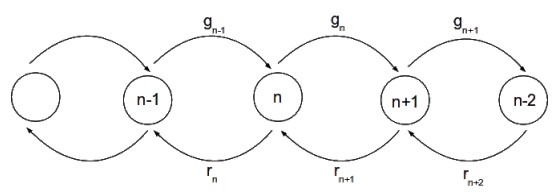
\includegraphics[scale=0.90]{theonestep.jpg}
\caption{ The one-step process with its transition probabilities and the different states. Image from \cite{Ragazza}.}
\label{theonestep}
\end{figure}
\newline 
Thus the master equation for one-step processes can be rewritten as
\begin{equation}\label{theonestepmasterequation}
\frac{dP_{n}(t)}{dt} = \dot{P_{n}} = r_{n+1}P_{n+1} + g_{n-1}P_{n-1}-(r_{n}+g_{n})P_{n}
\end{equation}
However, we need to beware to the boundary conditions. Given that we have a number of molecules \emph{n} that is $n \in [0,N]$, if $n = 0$ is a boundary, the Eq \ref{theonestepmasterequation} is meaningless and has to be replaced with 
\begin{equation}
\dot{P_{0}} = r_{1}P_{1} - g_{0}P_{0}
\end{equation}
since we need to set this condition $r_{0} = g_{-1} = 0$ otherwise we would have a negative number of molecules which is physically unfeasible. Similarly an upper boundary $n = N$ requires a special equation:
\begin{equation}
\dot{P_{N}} = g_{N-1}P_{N-1} - r_{N}P_{N}
\end{equation}
because the condition $r_{N+1}=g_{N}=0$ or then with $g_{N}$ we would have a transition from the state \emph{N} to the state $N+1$ and so to a state whose number of molecules is greater than the maximum number present in our system; a similar reasoning is done for $r_{N+1}$ that means a transition from the state $N+1$ to \emph{N}.


One-step processes can be subdivided based on the coefficients $r_{n}$ and $g_{n}$ into the following categories: linear, if the coefficients are linear functions of \emph{n}, nonlinear, if the coefficients are nonlinear functions of \emph{n} and random walks, if the coefficients are constant \cite{Ragazza,Math}.
\newline
An important example of a one-step process with constant transition probabilities is the \emph{Poisson process}, defined by
\begin{align}
    r_{n} = 0,g_{n}=q,p_{n}(0)=\delta_{n,0},
\end{align}
where \emph{q} is constant parameter. In such case, the master equation is
\begin{equation}
    \dot{P_{n}} = q(P_{n-1}-P_{n})
\end{equation}
The solution of this equation is a time dependent probability distribution
\begin{equation}
    P_{n}(t) = \frac{(qt)^{n}}{n!}e^{-qt}
\end{equation}
that is a Poisson distribution.


\section{Probability distributions in protein synthesis}
In this thesis, we will refer to reactions occuring inside a cell volume between different types of biochemical molecules with various reaction rates. These will generally be genes , i.e. sections of DNA that are copied into mRNA and initiate a gene expression network, RNA or proteins. As mentioned in section \ref{theonestepdiscussion}, such molecular reactions are random Poissonian birth-death processes. More rigorous theoretical efforts also invoke a simple birth–death model of transcription (the copying of a section of DNA to mRNA) and translation (protein production from mRNA), the analysis of which yields \emph{a scaling law}. For mRNA these depend on the type of regulation, with constitutive expression producing a Poisson distribution, as expected for a single birth-death process, and more complicated regulation strategies producing non-Poisson mRNA distributions. Proteins also have non-Poisson distributions (albeit their scaling is also roughly Poissonian), as they are dependent on both mRNA birth and death as well as translation rates \cite{Article}.


Experimental studies have confirmed these results, finding that total noise does scale roughly as the inverse square of abundance (namely, the number of molecules in the system) untill high abundances. At this point, extrinsic noise is thought to take over as the dominant source of noise.

\section{Resolution Methods for the CME}

Solving the master equation would seem to be the ideal way of looking at stochastic systems, as it can tell us the full distribution of possible states the system can be in over time, but for one important disadvantage: its complexity. This becomes apparent when considering how many equations must be solved at each time point, and bearing in mind that the number of possible states can increase exponentially with time \cite{Article}. 
 

Thus we must use trajectory-based approaches, which differ from the master equation in that they do not find the distribution of all possible states over time. Rather, \emph{they simulate single realizations}, meaning that at each step they choose one out of all the possible outcomes.


The trajectory of each stochastic simulation is different, since each is a single realisation sampled randomly from the full distribution given by the master equation. Given many of these random single trajectories, we can build up a picture of the full distribution.


Many approximation methods for the solution of the CME have been developed during the years. In this thesis, we will exploit the two algorithms that have become the workhorse stochastic methods for many researchers today: the stochastic simulation algorithm and the tau-leap simulation.

\subsection{Stochastic simulation algorithm}
Most of the attempts in solving the CME have concentrated on Monte Carlo simulations using the \emph{stochastic simulation algorithm} (SSA) proposed by Gillespie in his seminal paper. This method is statistically exact, namely a full probability distribution built up from an infinite number of simulations will be identical to the distribution of the Markov process, given by the master equation \cite{Article}. This algorithm is arguably the simplest SSA variant and is based on the following steps in order to simulate \emph{one stochastic realisation}: assuming that the system is described by the state vector $\Vec{Y}$ which in general represents the amount of molecules for each chemical species and given that the initial state of the system is $\Vec{Y} = \Vec{Y}_{0}$, one has to choose which reaction happens between the possible ones and how much time the system will spend in such state before the next reaction happens \cite{PHD}. Each reaction \emph{i} is described by its \emph{transition rate} (or even called \emph{propensity}) $k_{i}$ and by the modification of the state vector that generate. Given that we are dealing with Markov process, the difference in time between two successive events $\Delta t$ follows an \emph{exponential distribution}, whose parameter is the propensity $k_{i}$:
\begin{equation}
    p_{i}(\Delta t) = e^{-k_{i}\Delta t}
\end{equation}
given that any reaction is independent from the others, the distance in time between two successive events is distributed as:
\begin{equation}
    p(\Delta t) = e^{-\sum_{i=0}^{R} k_{i} \Delta t}
\end{equation}
This process is iterated untill the whole time of interest has been simulated.


Unfortunately, the direct method SSA pays the price for its simplicity in computational time, as two random numbers must be generated at each step \cite{Article} (the one for choice of the event and the other for the choice of the time spent in the state). Furthermore, the SSA has an inherent limitation: it must simulate every single reaction. This is, of course, its great strength too, but in cases where there are many reactions or larger molecular populations, it often becomes too slow to generate useful numbers of simulations in a practical time period.

\subsection{Tau-leap}
The tau-leap method is similar to the SSA in that each simulation is a \emph{single stochastic realisation} from the full distribution at each step. However, the steps are much larger (hence its name) \cite{Article} and in each one of these \emph{it counts the total number of occurrences of each type of reaction over that step}. Thus, also in this case based on the initial state of molecular populations $\Vec{Y}=\Vec{Y_{0}}$, if there are \emph{M} reactions, we take \emph{M} Poisson random number samples. We can call the time interval in which these reactions happen as $\tau$. Hence, the vector of molecules given by the \emph{M} reactions $\Vec{Y}=\Vec{Y}_{M}$ in the time interval $\tau$ is given by
\begin{equation}\label{MPoissonReactions}
    \Vec{Y}_{m}(\tau) = P(\Vec{K_{i}}\tau)
\end{equation}
where \emph{P} is the Poisson distribution with mean equal to $\Vec{K_{i}}\tau$ of which $\Vec{K_{i}}$ is the vector of propensities. Then the initial state of molecular populations is updated based on Eq \ref{MPoissonReactions}  and this is iterated untill the whole time of interest has been simulated, similarly to SSA.


Hence, the basic idea of this procedure is to advance the system by a \emph{pre-selected} time increment $\tau$ (in contrast to the generated time increment that is in the SSA), which is large enough that many reaction events occur in that time, but nevertheless small enough that \emph{no propensity function value is likely to change ``significantly'' as a consequence of those reaction events} \cite{Method}.


Summing all up, tau-leap algorithm has the key advantage that we now do not need to spend time simulating individual reactions and as such the it is much faster than the SSA. On the other hand its main drawback is that we have lost accuracy compared to the SSA in some ways such as we do not know exactly how many reactions occurred (we can only estimate this) and we do not know exactly when each reaction occurred within the time step.


The accuracy issue can be mitigated (at the expense of computational time) as the error level, and so time step size, is decreased; indeed, as the time step tends to zero, the tau-leap effectively becomes the SSA, with each step experiencing either zero or one reaction \cite{Article}. 


Finally, as anticipated in some rows above, there is another complementary issue with the tau-leap: as many reactions are simulated at once, molecular species that are depleted in any reaction can go negative if the time step is too large. This is obviously unphysical, and so undesirable, and schemes have been developed that allow the choice of larger time steps whilst avoiding negative populations \cite{Article}.
\section{Statistical analysis techniques for warm-up detection}

\section{Absorbing states}

\chapter{The NF-$\kappa$B family of transcription factors}
Nuclear factor kappa-light-chain-enhancer of activated B cells (abbreviated as NF-$\kappa$B) was first described as a transcription factor that regulates the expression of the kappa light chain of immunoglobulins \cite{YoutubeNFkB}.  It comprises a family of structurally-related eukaryotic transcription factors, which bind to consensus DNA sequences at promoter regions of responsive genes regulating a large number of normal cellular and organismal processes such as immune and inflammatory responses, developmental processes, cellular growth and apoptosis and, as such, this protein complex can be considered a pleiotropic mediator of gene expression control. There are five proteins in the mammalian NF-$\kappa$B family including NF-$\kappa$B1 (also named p50), NF-$\kappa$B2 (also named p52), RelA (also named p65), RelB and c-Rel. All proteins of the NF-$\kappa$B family share a \emph{Rel homology domain} (RHD). The RHD is composed of two structural domains: the N-terminal \emph{DNA binding domain} and the C-terminal domain that has an immunoglobulin-like fold that functions as a \emph{dimerisation domain} \cite{domain}. Hence, RHD is required for binding to spiecific DNA binding sites in the promoters of target genes and serves as a dimerization interface to other NF-$\kappa$B transcription factors since these members combine to form different dimers that regulate the transcription of target genes. %In addition, binds to the inhibitory I$\kappa$B$\alpha$ protein. 
\newline
In unstimulated cells, NF-$\kappa$B proteins are sequestered in the cytoplasm through binding to inhibitory molecules (i.e. the I$\kappa$Bs family) whose prototype is I$\kappa$B$\alpha$. Stimulation with a variety of stimuli, such as proinflammatory cytokines (e.g., TNFa and IL-1b), Toll-like receptor ligands [e.g., lipopolysaccharide (LPS) and double-stranded RNA (dsRNA)], triggers NF-$\kappa$B activation through the so called ‘classical’ or ‘canonical’ pathway. This signaling pathway leads to the IKK complex, composed of both kinases IKK$\alpha$ and IKK$\beta$ assembled by the scaffold protein NEMO/IKK$\gamma$. The IKK complex phosphorylates IkB$\alpha$ on N-terminal serines, and this triggers its degradative polyubiquitination through the proteasome (a simple sketch of this process is shown in figure \ref{NFkBactivation}). 

\begin{figure}
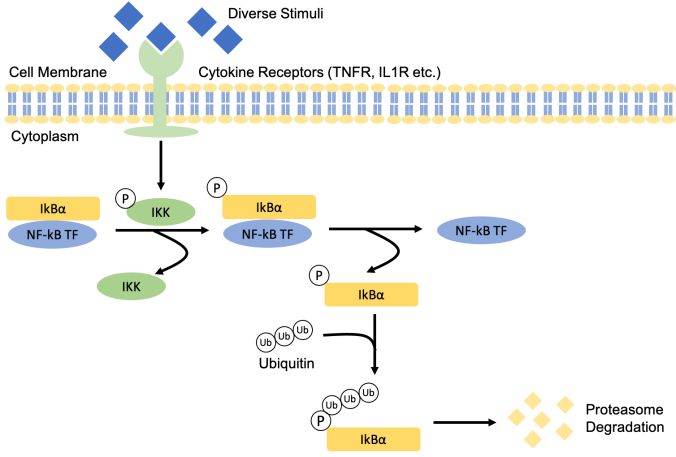
\includegraphics[scale=0.70]{NFkBactivation.png}
\caption{The binding of pro-inflammatory cytokines to its receptors triggers the activation of IKK which will phosphorylate IkB$\alpha$ releasing the sequestered NF-$\kappa$B Transcription Factor. The IkB$\alpha$ will then undergo proteasome degradation to synthesize new proteins. Image from \cite{Project}.}
\label{NFkBactivation}
\end{figure}
\newpage
NF-$\kappa$B dimers (mainly p50/p65, that is the major NF-$\kappa$B dimer of the canonical pathway, and p50/c-Rel) are consequently released and translocated to the nucleus to drive gene transcription of candidates involved in innate immunity, inflammation, proliferation, and survival (see figure \ref{NFkBmechanism}). 
\newline    
NF-$\kappa$B also activates transcription of the mRNA encoding its inhibitory subunit I$\kappa$B, thus generating a negative feedback circuit.

\begin{figure}[ht]
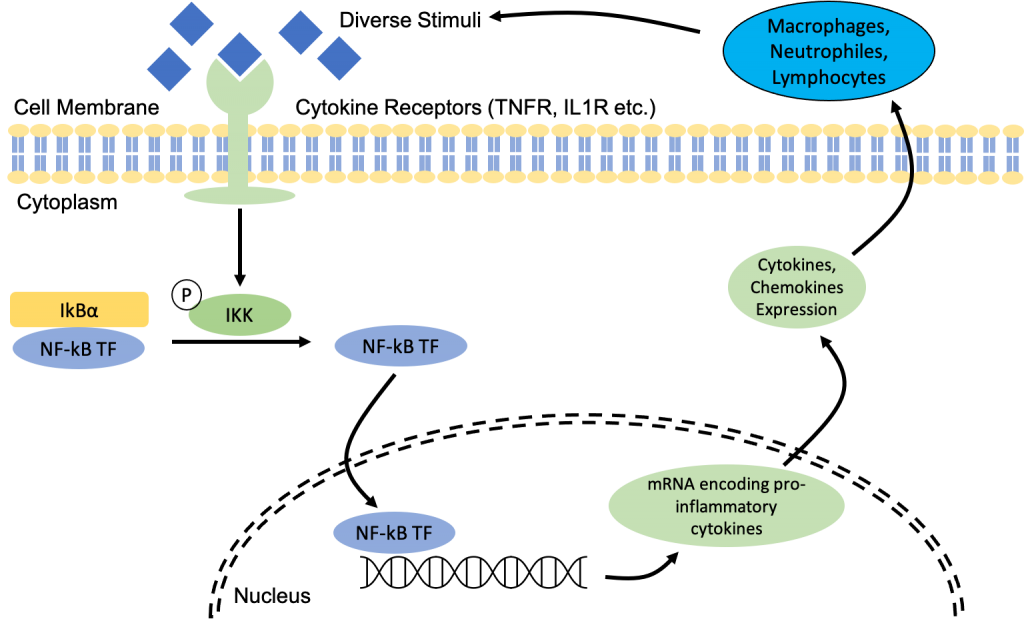
\includegraphics[scale=0.45]{NFkBmechanism.png}
\caption{NF-$\kappa$B will induce transcription expression of pro-inflammatory cytokines when bound to DNA. Pro-inflammatory cytokines will recruit immune cells to the site. Presence of immune cells further produces pro-inflammatory cytokines which could bind to the cytokine receptors that are responsible for activating NF-$\kappa$B. Image from \cite{Project}.}
\label{NFkBmechanism}
\end{figure}
\newpage
The ‘alternative’ or ‘non-classical’ NF-$\kappa$B-activating pathway is triggered by cytokines such as BAFF and lymphotoxin-b, and leads to the activation of an IKK$\alpha$ homodimer, which phosphorylates p100. This inhibitory molecule is subsequently processed to generate p52. NF-$\kappa$B dimers (p52/RelB) move into the nucleus to drive the expression of candidates involved in adaptive immunity, as well as in lymphoid organogenesis.


Finally, growth factors can also trigger the activation of the IKK complex through signaling pathways described in figure \ref{NFkBEGFR}.

\begin{figure}[ht]
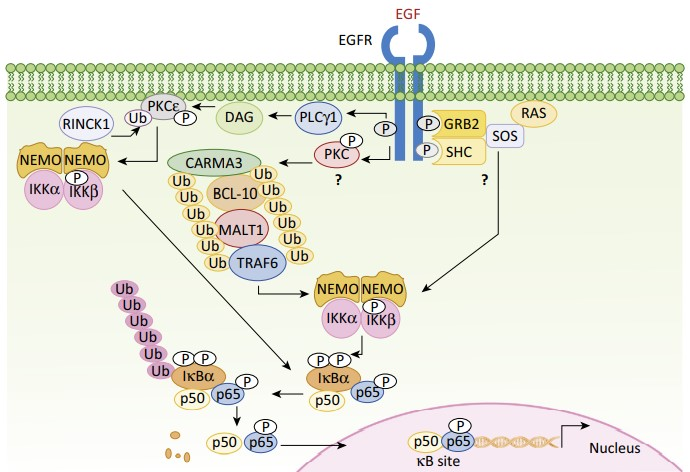
\includegraphics[scale=0.90]{EGFR.jpg}
\caption{Molecular mechanisms by which EGFR activates NF-kB. Image from \cite{EGFRNFkB}.}
\label{NFkBEGFR}
\end{figure}
Growth factor is a substance made by the body that functions to regulate cell division and cell survival \cite{GF}. Epidermal growth factor (EGF) is a protein that stimulates epidermal and epithelial cell growth and differentiation by binding to its receptor called Epidermal Growth Factor Receptor (EGFR) \cite{EGF}. The epidermal growth factor receptor is a transmembrane protein that is involved in cell signaling pathways that control cell division and survival \cite{EGFR}. Although it is now well established that EGF activates NF-$\kappa$B through the IKK complex, signaling molecules that link EGFR activation to the IKK complex have only been recently characterized.
\newpage
Hence, as said at the beginning, NF-$\kappa$B proteins are involved in the control of a large number of normal cellular and organismal processes. However, on the other hand, these transcription factors are persistently active in a number of disease states, including cancer, arthritis, chronic inflammation, asthma, neurodegenerative diseases, and heart disease \cite{NFkB}. In particular, constitutive epidermal growth factor receptor and nuclear factor $\kappa$b activities are seen in multiple solid tumors and combine to provide oncogenic signals to cancer cells. Recent studies have also defined mechanisms by which resistance occurs through crosstalk between EGFR- and NF-$\kappa$B-dependent pathways in colon cancer cells.


\addcontentsline{toc}{chapter}{Bibliography} %Adding the bibliography to contents.

\begin{thebibliography}{bibliography}
     \bibitem{Brizi} Gastone Castellani, teaching material of {\em Physical Methods of Biology} course, University of Bologna.
    \bibitem{PR} Daniel Remondini, Gastone Castellani, teaching material of {\em Pattern Recognition} course, University of Bologna.
    \bibitem{SDAFAP} Claudia Sala, Maximiliano Sioli, teaching material of {\em Statistical Data Analysis for Applied Physics} course, University of Bologna.
    \bibitem{SACFAP} Enrico Giampieri, teaching material of {\em Software and Computing for Applied Physics} course, University of Bologna.
    \bibitem{PHD} Giampieri Enrico, {\em Stochastic models and dynamic meaures for the characterization of bistable circuits in cellular biophysics}, University of Bologna (2012).
    \bibitem{Tesi} Davide Giosué Lippolis, {\em Stochastic modeling of fluctuations in the NF-$\kappa$B activity of neoplastic cells}, University of Bologna (2018/2019).
    \bibitem{Genetics} Yifeng Xia, Shen Shen, and Inder M. Verma, {\em NF-$\kappa$B, an active player in human cancers}, Cancer Immunol Res (2014) 2 (9): 823–830.
    \bibitem{NFkB} NF-kB Transcription Factors. URL \url{https://www.bu.edu/nf-kb/}.
    \bibitem{domain} Rel homology domain (RHD), DNA-binding domain. URL \url{https://www.ebi.ac.uk/interpro/entry/InterPro/IPR011539/}.
	\bibitem{Wiki} NF-kB. URL \url{https://en.wikipedia.org/wiki/NF-%CE%BAB}.
    \bibitem{Article} Tamás Székely Jr., Kevin Burrage, {\em Stochastic simulation in systems biology}, Computational and Structural Biotechnology Journal, Volume 12, Issues 20–21, November 2014, Pages 14-25.
    \bibitem{Method} Yang Cao, Daniel T. Gillespie and Linda Petzold, {\em Avoiding Negative Populations in Explicit Poisson Tau-Leaping}, Article  in  The Journal of Chemical Physics, September 2005.
    \bibitem{Project} INFLAMMATION'S ROLE IN OBESITY. URL \url{https://sites.tufts.edu/hkerstjaaalislai/?page_id=541}.
    \bibitem{EGFRNFkB} Kateryna Shostak and Alain Chariot, {\em EGFR and NF-kB: partners in cancer}, Trends in Molecular Medicine June 2015, Vol. 21, No. 6.
    \bibitem{YoutubeNFkB} NF-$\kappa$B pathways, Part 1: The canonical pathway of NF-$\kappa$B activation. URL \url{https://www.youtube.com/watch?v=7F_HPRfHdDk}.
    \bibitem{Definition} Genetic Heterogeneity. URL \href{https://www.sciencedirect.com/topics/biochemistry-genetics-and-molecular-biology/genetic-heterogeneity}{https://www.sciencedirect.com/}
    \bibitem{EGFR} epidermal growth factor receptor. URL \href{https://www.cancer.gov/publications/dictionaries/cancer-terms/def/epidermal-growth-factor-receptor}{https://www.cancer.gov}
    \bibitem{GF} growth factor. URL \href{https://www.cancer.gov/publications/dictionaries/cancer-terms/def/growth-factor}{https://www.cancer.gov}
    \bibitem{EGF} Epidermal growth factor. URL \href{https://en.wikipedia.org/wiki/Epidermal_growth_factor}{https://en.wikipedia.org}
    \bibitem{Math} N. G. van Kampen, {\em Stochastic Processes in Physics and Chemistry}, North Holland, third ed., May 2007.
    \bibitem{ACF} Autocorrelation Function. URL \href{https://www.sciencedirect.com/topics/chemistry/autocorrelation-function#:~:text=1%20Autocorrelation-,The%20autocorrelation%20function%20(ACF)%20defines%20how%20data%20points%20in%20a,signal%20over%20different%20delay%20times.}{https://www.sciencedirect.com}
    \bibitem{Stat} G. Cowan, {\em Statistical Data Analysis}, Oxford University Press Inc., New York, 1998.
    \bibitem{onesteparticle} Mathisca de Gunst, Michel Mandjes and Birgit Sollie, {\em Statistical inference for a quasi birth–death model of RNA transcription}, BMC Bioinformatics 23, 105 (2022).
    \bibitem{Hand} C.W.Gardiner, {\em Handbook of Stochastic Methods for Physics, Chemistry and the Natural Sciences}, Printed in Germany, Springer-Verlag Berlin Heidelberg 1983,1985.
    \bibitem{Ragazza} Luciana Renata De Oliveira, {\em Master Equation: Biological Applications and Thermodynamic Description}, University of Bologna (2013/2014).


\end{thebibliography}








\end{document}

